
\textbf{Heston model prices} produced by the market\!\,\footnote{
The fit uses 271 calibration cells across 8 maturities and 91 strikes,
backed by 163,016 contracts of traded volume.
The reference spot was $S_{\mathrm{ref}} = 1358.1765$,
priced under a risk-free rate of 0.17\% and a dividend rate of 2.06\%.
The intraday spot range was 1.23\%.
Fit quality is 0.65 vol points of implied-volatility RMSE,
with a relative-price RMSE of 0.1512.
The Feller condition violates at this calibration,
with $2\kappa\theta - \eta^2 = -0.8528$.
} 
calibrated pricing operator:
\begin{center}
    $C_{\mathrm{H}}(\Phi^{\star}; S,K,\tau,w)$~\eqref{eq:heston-price}~\eqref{eq:accept}.
\end{center}
\begin{figure}[H]
    \begin{center}
        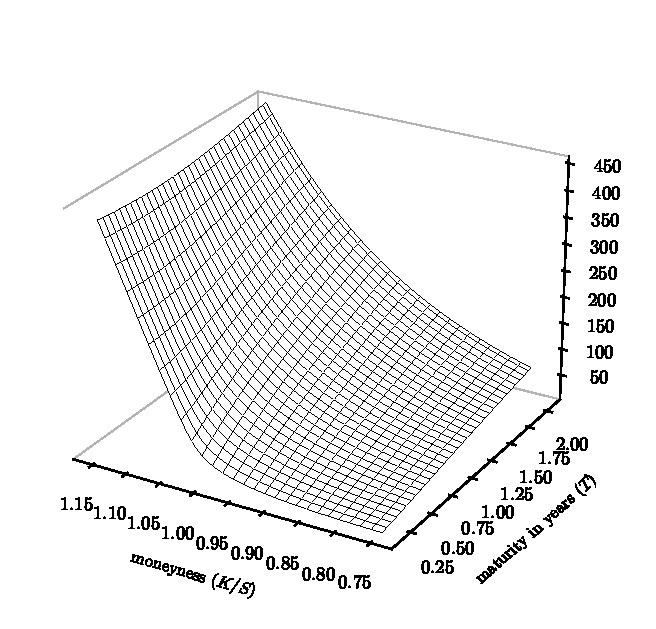
\includegraphics[width=6.25cm,keepaspectratio=true]{results/heston/surfaces/plots/tex/price_surface_puts.eps}
        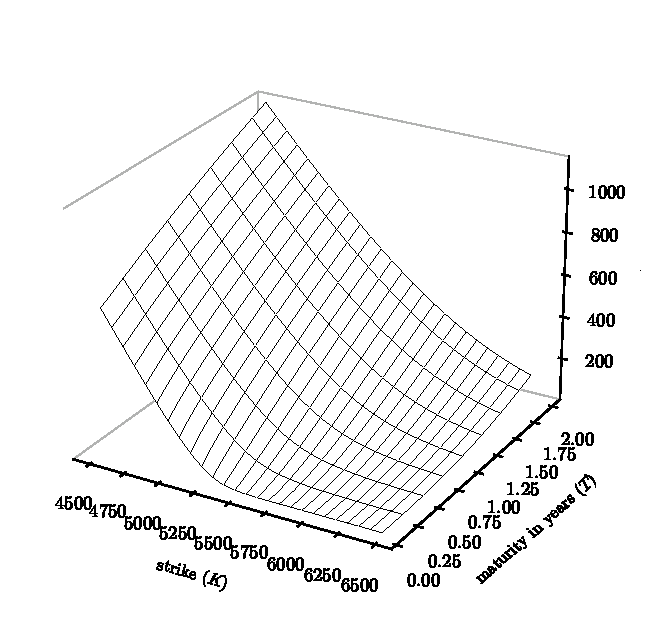
\includegraphics[width=6.25cm,keepaspectratio=true]{results/heston/surfaces/plots/tex/price_surface_calls.eps}
        \caption{Heston option prices for $S_{\mathrm{ref}}$ 1358.1765 on May 11, 2012 with $\Phi^{\star} = (0.1302,\ 1.0255,\ 1.0582,\ -0.7401,\ 0.034)$: puts wing (left) and calls wing (right).}
        \label{Fig:wings}
    \end{center}
    \begin{center}
        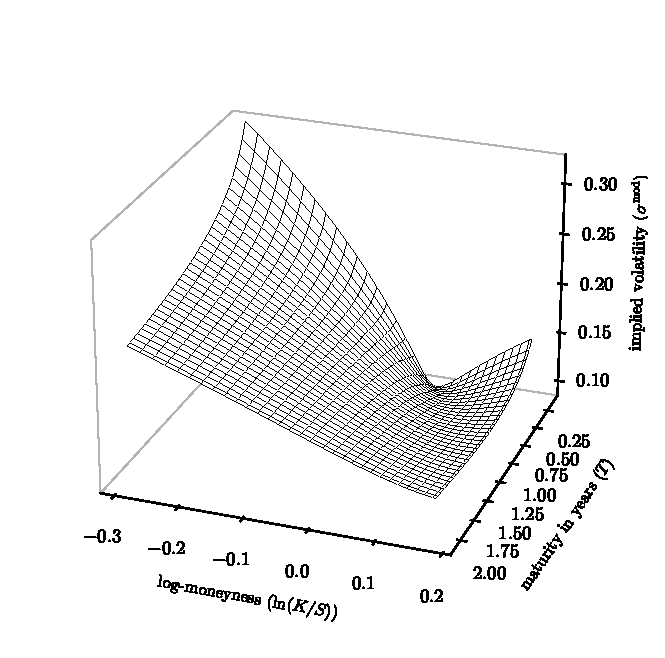
\includegraphics[width=9cm,keepaspectratio=true]{results/heston/surfaces/plots/tex/smile_surface.eps}
        \caption{\emph{Out of the money} implied volatilites from Figure~\ref{Fig:wings}}
    \end{center}
\end{figure}

